\chapter{How to Crush Sales}

This chapter is based on a School of Hard Knocks entrepreneurship interview curated by LazyingArt LLC. The exchange is brief, but it unfolds with a clear internal logic. We begin with the buyer's resistance to being sold, then move to the method the speaker calls solution selling: ask questions, find the real need, decide whether the offer fits, and only then present the solution. The source gives no blackboard equations or diagrams, so the notation below is a disciplined reconstruction of the spoken argument, not an added theory.

\section{Selling Without Pressure}

The opening question is: how could someone crush sales in 2022? The answer does not begin with a script or a close. It begins with a constraint on the buyer.

\begin{equation}
\text{People dislike being sold to,}
\qquad
\text{but people still like to buy.}
\end{equation}

This is the little paradox that drives the lecture. If we push, the buyer resists. If we help the buyer recognize and solve a real problem, the buyer can move toward the purchase by choice.

A simple way to write the bad path is

\begin{equation}
\text{seller pressure}
\;\longrightarrow\;
\text{buyer resistance}.
\end{equation}

The useful path has a different order:

\begin{equation}
\text{buyer need}
\;\longrightarrow\;
\text{relevant solution}
\;\longrightarrow\;
\text{buyer decision}.
\end{equation}

The difference is not cosmetic. In the first case, the seller is trying to move the buyer. In the second, the seller is trying to understand what would make movement rational for the buyer.

\subsection{Question \& Answer}

\paragraph{Question.}
If no one likes to be sold to, how can sales work at all?

\paragraph{Answer.}
Sales works when it stops being pressure first and becomes diagnosis first. The buyer is not asked to surrender to a pitch. The buyer is helped to clarify a need, name a pain point, and decide whether the seller has something that actually helps.

So the first principle is not ``talk better.'' It is ``learn first.''

\begin{equation}
\text{ask}
\;\longrightarrow\;
\text{understand}
\;\longrightarrow\;
\text{offer only if useful}.
\end{equation}

That is the rhythm of the rest of the lecture.

\section{Solution Selling}

The speaker gives the method a name: solution selling. He also says there are many names for it, which keeps us from treating the label as the lesson. The lesson is the order of operations.

Let \(N\) be the buyer's true need, and let \(S\) be a proposed solution. A seller who starts with \(S\) before discovering \(N\) has reversed the problem. The disciplined sequence is

\begin{equation}
\text{questions}
\;\longrightarrow\;
N
\;\longrightarrow\;
\text{test whether } S \text{ helps}
\;\longrightarrow\;
\text{mutual problem-solving}.
\end{equation}

\begin{definition}
A \emph{solution-selling conversation} is a sales conversation in which the seller first asks questions, then identifies the buyer's need \(N\), and only after that decides whether a proposed solution \(S\) belongs in the conversation.
\end{definition}

This gives us a minimal fit relation:

\begin{equation}
\operatorname{Fit}(S,N)=
\begin{cases}
1, & \text{if } S \text{ helps solve } N,\\
0, & \text{if } S \text{ does not help solve } N.
\end{cases}
\end{equation}

\begin{remark}
This notation is only bookkeeping. The interview does not claim that selling is a formula. The notation preserves the speaker's sequence: do not present a solution before you know the problem it is supposed to solve.
\end{remark}

The phrase ``real true need'' matters here. It tells us that the first answer from the buyer may not be enough. We ask questions until the conversation uncovers what is actually causing the difficulty.

\section{Questions Before Claims}

The speaker then states the method in first-person practical terms: he sells by asking questions, understanding the real need first, and then seeing whether he can help. That is the diagnostic posture. The seller's first job is not performance. It is inquiry.

Let

\begin{align}
Q &:= \text{the questions asked of the client},\\
N(Q) &:= \text{the need revealed by those questions},\\
S &:= \text{the seller's possible solution}.
\end{align}

The operating rule is

\begin{equation}
\text{present } S
\quad
\text{only after } N(Q) \text{ is clear enough to test fit}.
\end{equation}

So we should not imagine the sales conversation as a monologue. It is closer to an update process:

\begin{equation}
Q_1,Q_2,\ldots,Q_k
\;\longrightarrow\;
N(Q_1,\ldots,Q_k)
\;\longrightarrow\;
\operatorname{Fit}(S,N).
\end{equation}

The seller asks, listens, and updates the picture of the client. Only then can the seller know whether the offer is relevant.

\begin{figure}
\centering
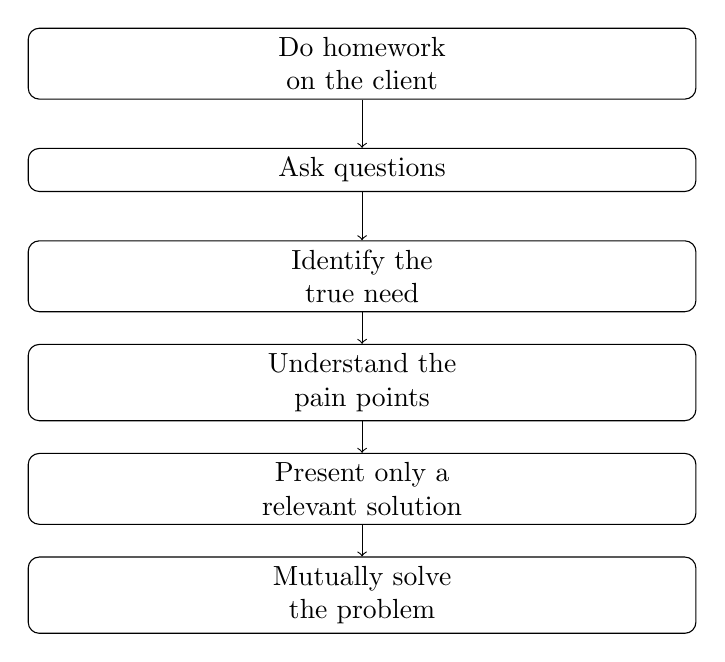
\begin{tikzpicture}
\node[draw, rounded corners, align=center, text width=0.68\linewidth] (a) at (0,0) {Do homework\\on the client};
\node[draw, rounded corners, align=center, text width=0.68\linewidth] (b) at (0,-1.35) {Ask questions};
\node[draw, rounded corners, align=center, text width=0.68\linewidth] (c) at (0,-2.70) {Identify the\\true need};
\node[draw, rounded corners, align=center, text width=0.68\linewidth] (d) at (0,-4.05) {Understand the\\pain points};
\node[draw, rounded corners, align=center, text width=0.68\linewidth] (e) at (0,-5.40) {Present only a\\relevant solution};
\node[draw, rounded corners, align=center, text width=0.68\linewidth] (f) at (0,-6.75) {Mutually solve\\the problem};
\draw[->] (a) -- (b);
\draw[->] (b) -- (c);
\draw[->] (c) -- (d);
\draw[->] (d) -- (e);
\draw[->] (e) -- (f);
\end{tikzpicture}
\caption{A narrow reconstruction of the spoken sequence: preparation, questioning, need discovery, pain-point focus, relevant presentation, and mutual problem-solving.}
\end{figure}

\section{The Demo-First Failure Mode}

Once the speaker has given the positive method, he turns to the failure mode. A young salesperson comes in and says, in effect: let me show you everything I have; when you see something interesting, stop me.

\paragraph{Anecdote.}
The novice seller leads with the demo. The buyer is expected to watch a broad presentation and identify the useful part.

\paragraph{Claim.}
That is the wrong order. The buyer is being asked to do the seller's diagnostic work.

In notation, demo-first selling begins with the seller's inventory,

\begin{equation}
S_1,S_2,S_3,\ldots,
\end{equation}

before the buyer's need \(N\) has been discovered. The seller is therefore hoping for an accidental match:

\begin{equation}
S_1,S_2,S_3,\ldots
\quad \text{shown before} \quad
N \text{ is known}
\quad
\approx
\quad
\text{random search}.
\end{equation}

The speaker's rough image is that this is like throwing things at a wall and seeing what sticks. We do not need to keep the coarse phrasing to preserve the point. The point is that undiagnosed presentation is low-discipline selling.

\begin{table}
\centering
\begin{tabular}{p{0.42\linewidth}p{0.42\linewidth}}
\textbf{Demo-first selling} & \textbf{Solution selling} \\
Starts with what the seller has & Starts with what the buyer needs \\
Shows many features early & Asks questions early \\
Waits for interest to appear & Identifies pain points first \\
Treats fit as accidental & Tests fit deliberately \\
Feels like pressure & Can feel like help \\
\end{tabular}
\caption{The lecture's core contrast: product-centered demonstration versus need-centered diagnosis.}
\end{table}

The table should be read vertically. The wrong method is not merely inefficient; it is pointed in the wrong direction. It starts from the seller's pile of offerings. The right method starts from the buyer's problem.

\section{Homework, Pain Points, And Fit}

After rejecting the demo-first method, the speaker makes the operational turn: slow down. Do homework on the client before showing up. He adds that few people do this, which makes preparation a practical advantage.

Let \(H\) denote homework on the client, and let \(P\) denote the pain points discovered or sharpened through that homework and questioning. The useful sequence is

\begin{equation}
H
\;\longrightarrow\;
Q
\;\longrightarrow\;
P
\;\longrightarrow\;
N
\;\longrightarrow\;
\operatorname{Fit}(S,N).
\end{equation}

This is not a separate system. It is solution selling made operational. Homework helps us ask better questions. Better questions reveal sharper pain points. Sharper pain points let us test whether the solution belongs.

\subsection{A Worked Fit Check}

Suppose the seller has a small set of possible features or offers,

\begin{equation}
S=\{s_1,s_2,s_3\},
\end{equation}

and suppose the client conversation reveals two pain points,

\begin{equation}
P=\{p_1,p_2\}.
\end{equation}

The demo-first seller presents all of \(S\) and waits. The solution seller builds a fit map:

\begin{equation}
F_{ij}=
\begin{cases}
1, & \text{if } s_i \text{ helps with } p_j,\\
0, & \text{otherwise.}
\end{cases}
\end{equation}

From that map we can define a relevance score for each possible offer:

\begin{equation}
r_i=\sum_j F_{ij}.
\end{equation}

The seller should present only the offers with positive relevance:

\begin{equation}
S_{\mathrm{present}}
=
\{\,s_i \in S : r_i>0\,\}.
\end{equation}

This is the clean mathematical version of the speaker's practical advice. We do not show everything. We show what touches the client's pain. If \(r_i=0\), then \(s_i\) may be a real feature, but it has not earned a place in this conversation.

The worked rule also explains why the homework comes before the meeting. Without \(P\), the seller cannot build \(F_{ij}\). Without \(F_{ij}\), the seller cannot distinguish a relevant solution from an irrelevant one. The meeting then collapses back into random demonstration.

\section{Mutual Problem-Solving}

The last movement of the lecture is the phrase ``mutually solve a problem.'' That is the payoff. The seller is not simply trying to move inventory, and the buyer is not simply being worked through a pitch. Both sides are now oriented toward the same object: the problem.

\begin{equation}
\text{selling as pressure}
\neq
\text{selling as joint problem-solving}.
\end{equation}

The contrast at the end is sharp. The speaker rejects trying to sell something opportunistically, like selling off the back of a truck. That image stands for low-trust, low-context selling. The solution-selling method stands for the opposite: context first, need first, fit first.

For the larger entrepreneurship book, this is the commercial principle worth carrying forward. Revenue is more durable when it comes from understanding the client's problem well enough to become useful. Sales, in this frame, is not just persuasion. It is judgment under commercial pressure.

\section{Summary}

The lecture gives a compact sales model. The buyer does not want pressure, but the buyer may want to buy. The seller's job is to discover the need, not to overwhelm the buyer with a demo.

The positive path is

\begin{equation}
\text{homework}
\;\longrightarrow\;
\text{questions}
\;\longrightarrow\;
\text{pain points}
\;\longrightarrow\;
\text{true need}
\;\longrightarrow\;
\text{fit}
\;\longrightarrow\;
\text{mutual solution}.
\end{equation}

The rejected path is

\begin{equation}
\text{show everything}
\;\longrightarrow\;
\text{hope something interests the buyer}
\;\longrightarrow\;
\text{weak selling}.
\end{equation}

The practical lesson is simple and demanding: strong selling is not louder persuasion. It is better diagnosis, followed by a solution that fits what the buyer actually needs.